\begin{frame}{Ré-appropriation de ces plateformes}
    \centering
    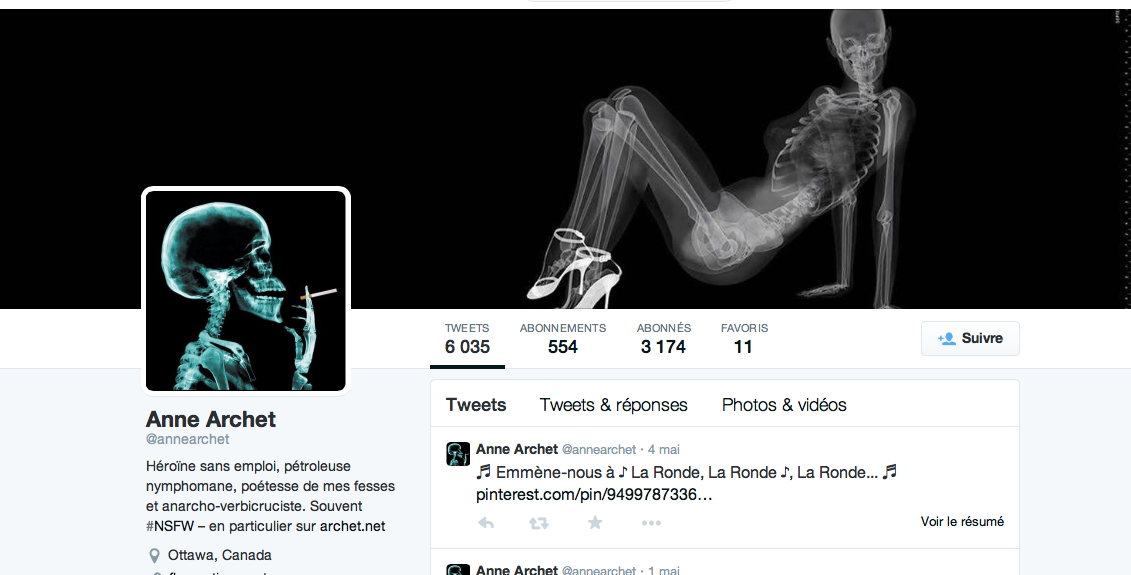
\includegraphics[width=.8\textwidth]{Images/AnneARchetTwitter.png}
\end{frame}

\begin{frame}{Ré-appropriation de ces plateformes}
    \centering
    
\includegraphics[width=.6\textwidth]{Images/generalInstinFB.png}
\end{frame}

\begin{frame}{Ré-appropriation de ces plateformes}
    \centering
    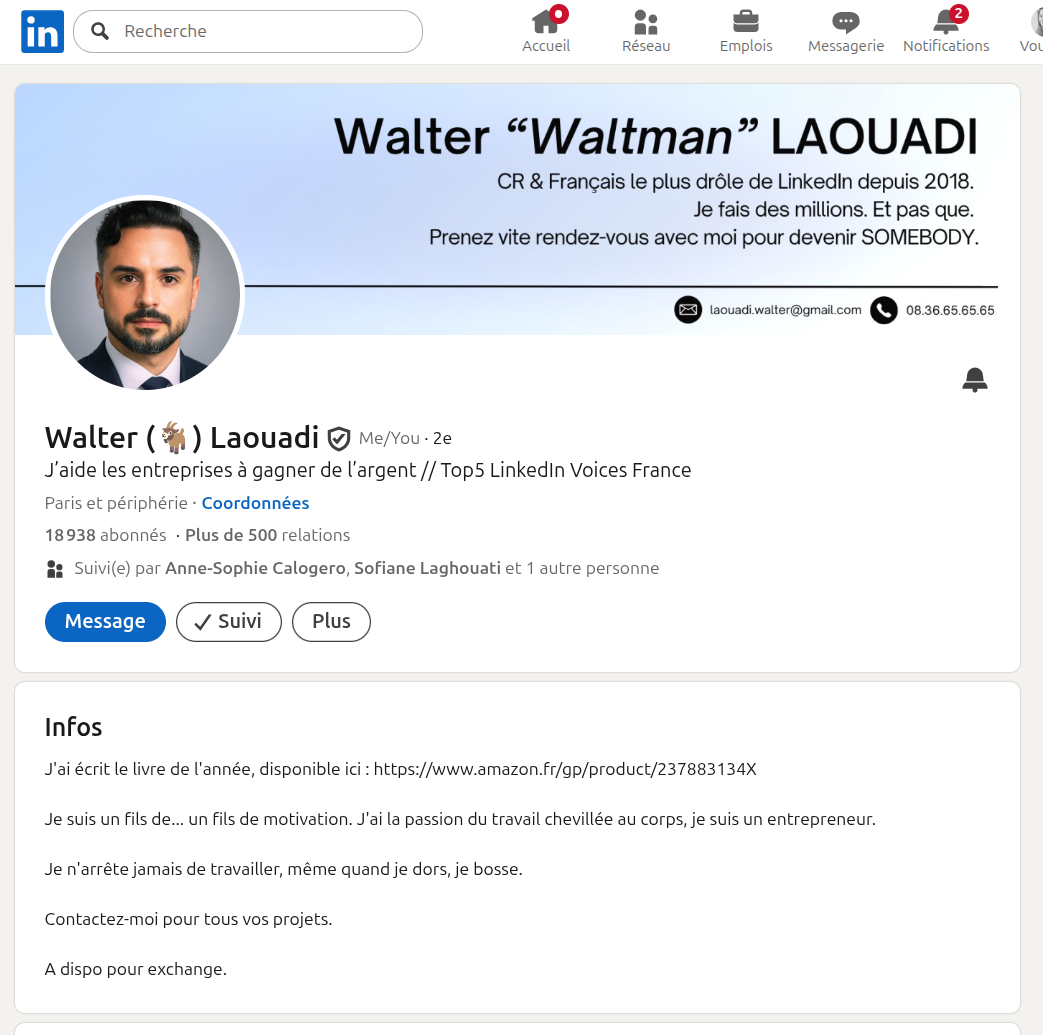
\includegraphics[width=.6\textwidth]{Images/walterLaouadi.png}
\end{frame}

\begin{frame}{La "maîtrise de la déprise" (Merzeau)}
    \begin{center}
        {\small \textit{La première protection contre "l'expropriation identitaire" [induite par les écritures numériques] consiste donc à reprendre la main sur la gestion de nos traces — en déposant un nom de domaine, en administrant un site, en agrégeant ses favoris… D'une façon générale, face à l'impossibilité de se soustraire aux systèmes de surveillance, où l'acteur enregistre lui-même les indices de sa présence, qui peut l'aider à préserver l'intégrité de son identité.}}
    \end{center}
    
\end{frame}

\begin{frame}{(Re)travailler ses données "personnelles"}
    \centering
    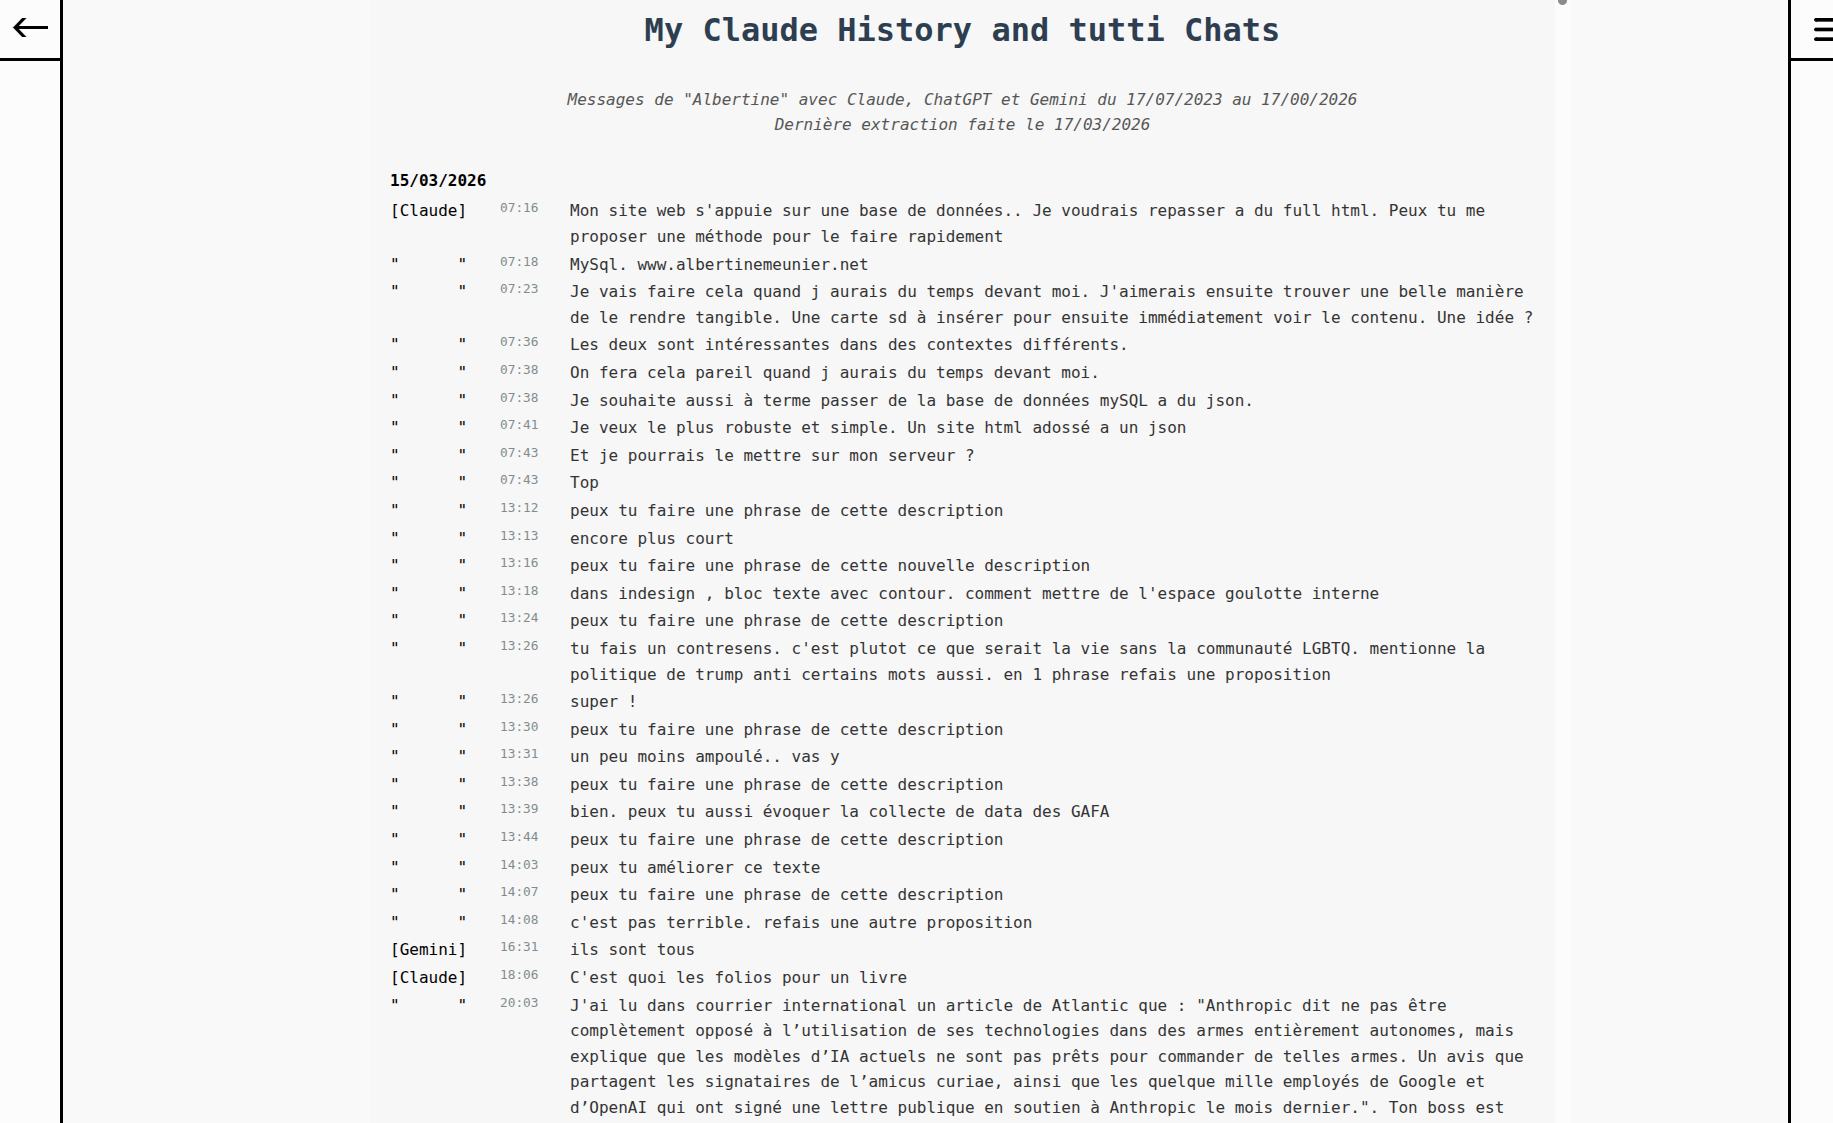
\includegraphics[width=.8\textwidth]{Images/albertine-Meunier-history-IA.png}
    
\end{frame}